
\chapter{Computing Performance \label{chpt:seq-code-performance}}

This section evaluates the computing performance (timing) of the code.
Our goal is to show that the new algorithm of angular convolution
is much faster than the old naive one; the huge amount of simulation
during this thesis has proven that to be the case. But a raw result,
where the implementation goes for an indefinite number of iterations
during minimization, cannot give a proper and systematic performance
evaluation. This is the purpose of this section.

In this section, we will evaluate the performance only within the
$\mathcal{F}_{\mathrm{exc}}$ term, knowing that other two terms takes
time of the same magnitude than the new algorithms for $\mathcal{F}_{\mathrm{exc}}$
part. The spatial and angular grid dependence of branches are discussed.

\section{FFT}

The \acs{FFT} play an important role in the implementation, which
is used by the spatial convolution and the \acs{FGSHT} process. 

\begin{figure}[H]
\begin{centering}
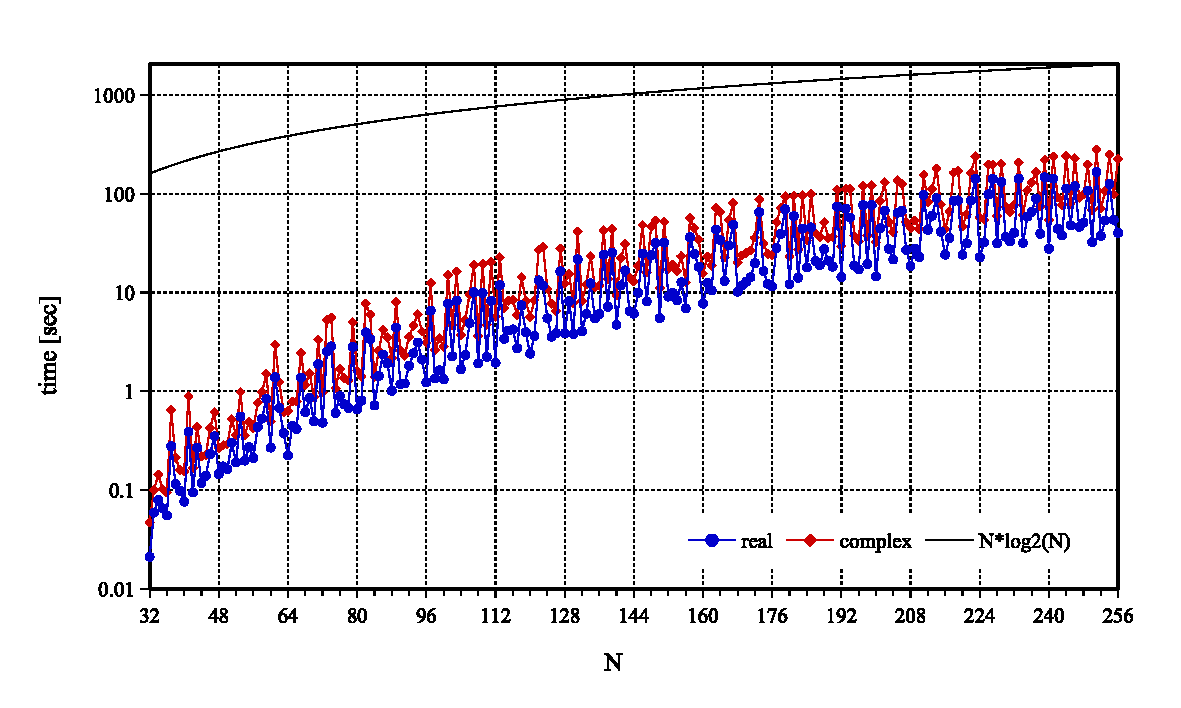
\includegraphics[bb=0bp 20bp 567bp 310bp,width=1\columnwidth]{_figure/results/fftw_timing}
\par\end{centering}
\caption{Timing of \acs{FFT} for real-to-complex and complex-to-complex processes
with respect to grid number $N$\label{fig:timing-FFT}}
\end{figure}

Referring to figure \ref{fig:timing-FFT}, the dependance on $O(N\log_{2}N)$
\citep{Numerical_Recipes_3ed} doesn't totally exist, but of the same
form, depending on the algorithm of \acs{FFT} \citep{Briggs-DFT}.
It should be noted that a grid of prime number is always at the peaks
in the figure, which means it can be 2 or more times longer than that
of the composite number around. Therefore it is better to use an even
number grid, where the $k$-border correction in $\mathsection$\ref{subsec:k-border-effect}
is absolutely involved in. Apart from this conclusion, to compare
between the algorithms for angular part involved in this thesis, we
are not really interested in computing performance with respect to
the number of spatial grid. However, the ratio of real and complex
\acs{FFT} timing is important, illustrated in figure \ref{fig:fft-real-to-complex},
where the ratio between real-to-complex and complex-to-complex \acs{FFT}
processes is 0.54, near the theoretical ratio 0.5. For example, we
process $n_{\mathrm{angle}}$ real to complex \acs{FFT}, then $n_{\mathrm{spatial}}/2$
complex to complex \acs{FGSHT}. Or we process $n_{\mathrm{spatial}}$
real to complex \acs{FGSHT}, then $n_{\mathrm{proj}}/2$ complex
to complex \acs{FFT}. This should not give a great difference if
$n_{\mathrm{angle}}\sim n_{\mathrm{proj}}$ for small $n_{\max}$.
If the the ratio is not 1:2, it will have an influence on the choice
of algorithm.
\begin{center}
\begin{figure}[h]
\begin{centering}
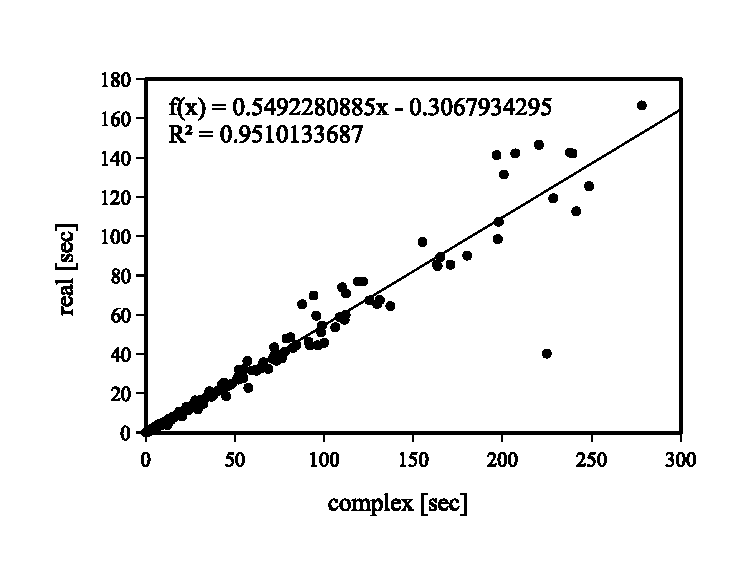
\includegraphics[bb=0bp 20bp 340bp 235bp,width=0.5\columnwidth]{_figure/results/fftw_real_v_cmplx}
\par\end{centering}
\caption{Timing of real-to-complex \acs{FFT} processes with respect to its
complex-to-complex process of the same grid number $N$\label{fig:fft-real-to-complex}}
\end{figure}
\par\end{center}

\section{FGSHT}

The computing times of \acs{GSHT} and \acs{FGSHT} are shown in figure
\ref{fig:time-gsht-fgsht}. There is no reason to see in detail how
much \acs{FFT} has accelerated the \acs{GSHT} process, but clearly
\acs{FGSHT} can be 100 times faster than \acs{GSHT}, and \acs{GSHT}
for the symmetry of $\Psi$, $s=1$ is on average 5 times longer than
$s=2$ ($s$ being the \acs{MRSO} defined in $\mathsection$\ref{sec:fgsht}).
As accuracy test shows that \acs{GSHT} and \acs{FGSHT} give exactly
the same result, and the case $m_{\max}<n_{\max}$ is never needed,
it is possible to utilize \acs{FGSHT} in all the cases to have a
faster performance.
\begin{center}
\begin{figure}[H]
\begin{centering}
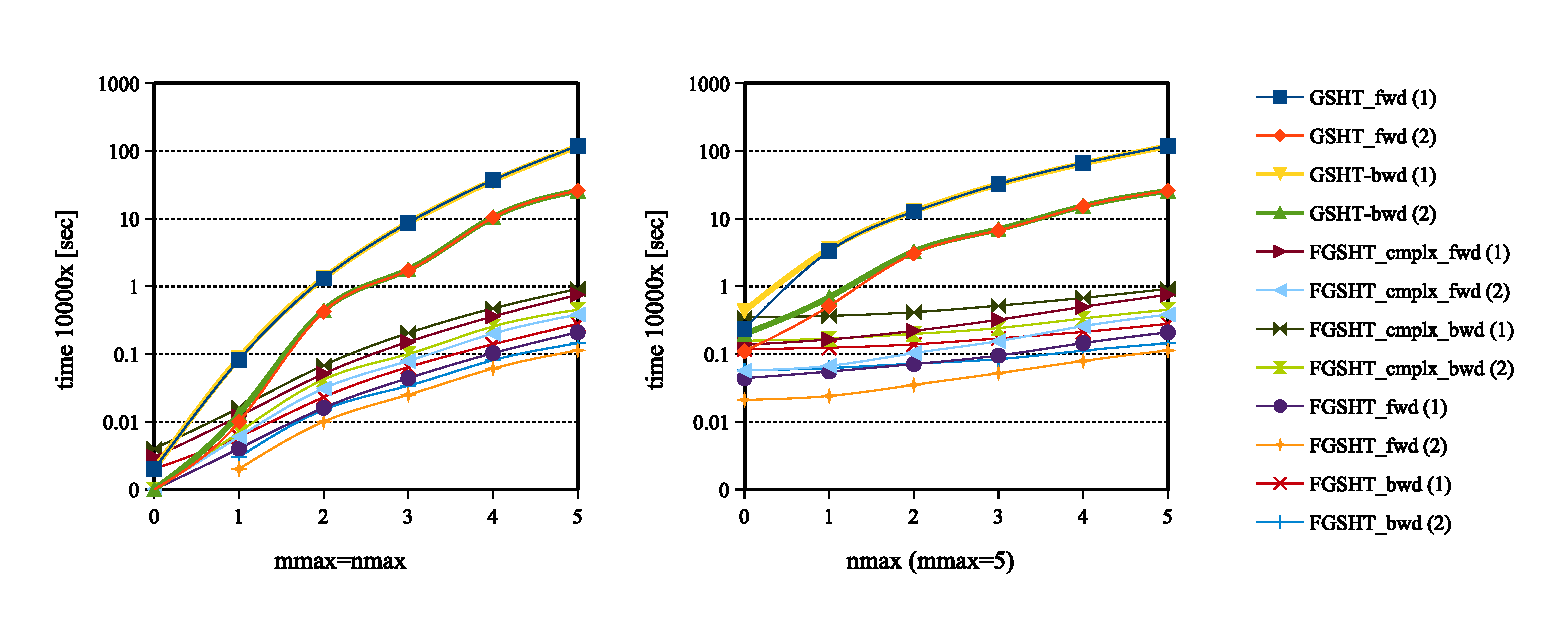
\includegraphics[bb=0bp 20bp 731bp 263bp,width=1\columnwidth]{_figure/results/fgsht_perf}
\par\end{centering}
\caption[Computing time of \acs{GSHT} and \acs{FGSHT}]{Computing time of \acs{GSHT} and \acs{FGSHT} (per 10000 times),
between parentheses is the order of symmetry axes $s$\label{fig:time-gsht-fgsht}}
\end{figure}
\par\end{center}

However, it is important to know the ratio between real and complex
\acs{FGSHT} processes for the same reason as \acs{FFT}. It is demonstrated
that this number is 0.3 in all cases, and it does not depend on $m_{\max}$,
$n_{\max}$ or $s.$ The difference between these two is that the
real one performs real-to-complex \acs{FFT} for the $\Phi,\Psi$
grid and calculates only slightly more than half of projections ($\mu\geq0$)
than the complex one.\textcolor{red}{{} }Theoretically, the ratio should
be greater than 0.5. This could mean there may be an extra process
in the complex one, or it is controlled by the memory. Ultimately,
the final result 0.3 means, that doing $n_{\mathrm{spatial}}$ real
to complex \acs{FGSHT} takes only 0.6 the time of doing $n_{\mathrm{spatial}}/2$
complex to complex \acs{FGSHT}, which means in \texttt{\textbf{convolution\_standard}}
we use less time to compute \acs{FGSHT} than in \texttt{\textbf{convolution\_pure\_angular}}.
\textcolor{red}{(Which is in fact not observed in the following tests.)}
\begin{center}
\begin{figure}[H]
\begin{centering}
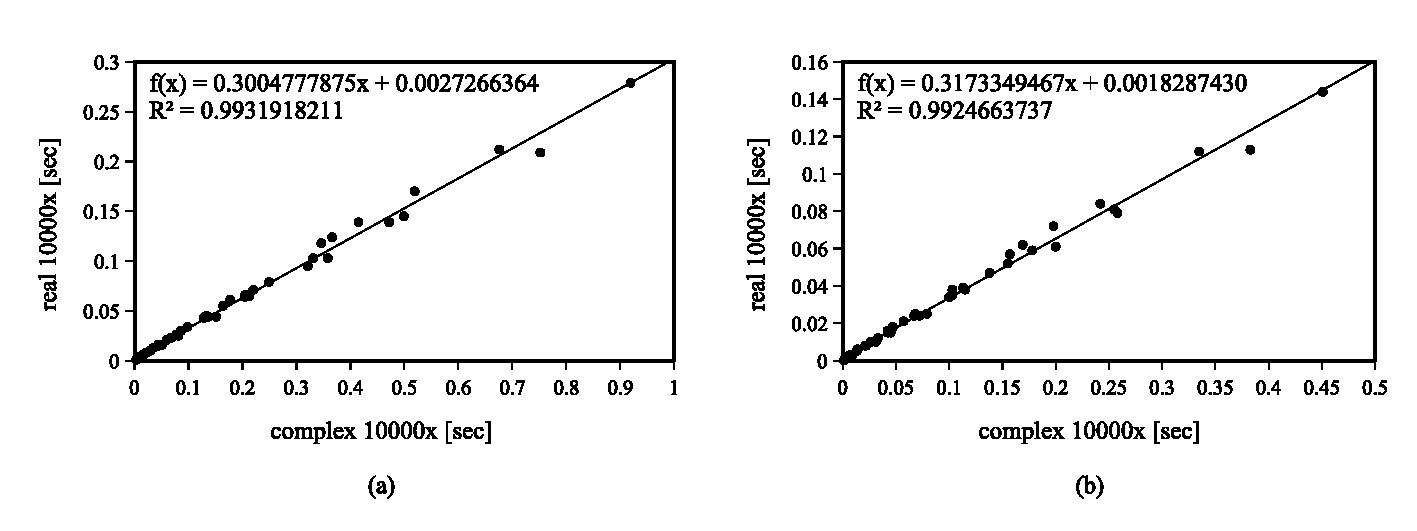
\includegraphics[bb=0bp 20bp 680bp 235bp,width=1\columnwidth]{_figure/results/fgsht_real_v_cmplx}
\par\end{centering}
\caption[Timing of real-to-complex \acs{FGSHT} processes with respect to its
complex-to-complex process of the same $m_{\max}$ and $n_{\max}$]{Timing of real-to-complex \acs{FGSHT} processes with respect to
its complex-to-complex process of the same $m_{\max}$ and $n_{\max}$,
for $s=1$ and $s=2$\label{fig:fgsht-real-to-complex}}
\end{figure}
\par\end{center}

\section{$k$-kernel\label{sec:-kernel}}

As discussed in the previous section, the final result of energy and
structure is independent of the choice of path inside a $k$-kernel.
That means we are free in terms of precision cost to choose the fast
path. Path (1) passed directly by $\hat{c}(k,\mathbf{\Omega}_{1},\mathbf{\Omega}_{2})$
in figure \ref{fig:k-kernel} has no interest in timing, as the memory
limit does not support such a direct algorithm for the entire $k$-space.
Here we only compare the paths (2), (3) and (4), which correspond
to eq. (\ref{eq:gamma-k}), (\ref{eq:im}) and (\ref{eq:gamma-blum}).

The theoretical predictions of the computing time of \acs{OZ} equation
with respect to $m_{\max}=n_{\max}$ are listed in table \ref{tab:FE-of-OZ}.
If the \acs{OZ} equation is the most time-consuming part, the result
should have the same proposal. Figure \ref{fig:Timing-k-kernel} shows
the experimental timing of the three paths, where path (3) is 100
times longer than (4), well corresponding to the theoretical value.
Path (2) is much longer than path (3) because apart from the \acs{OZ}
equation, the lecture and calculation of the \acs{DCF} mentioned
in $\mathsection$\ref{chpt:fft-spatial} also takes time.

\begin{figure}[H]
\begin{centering}
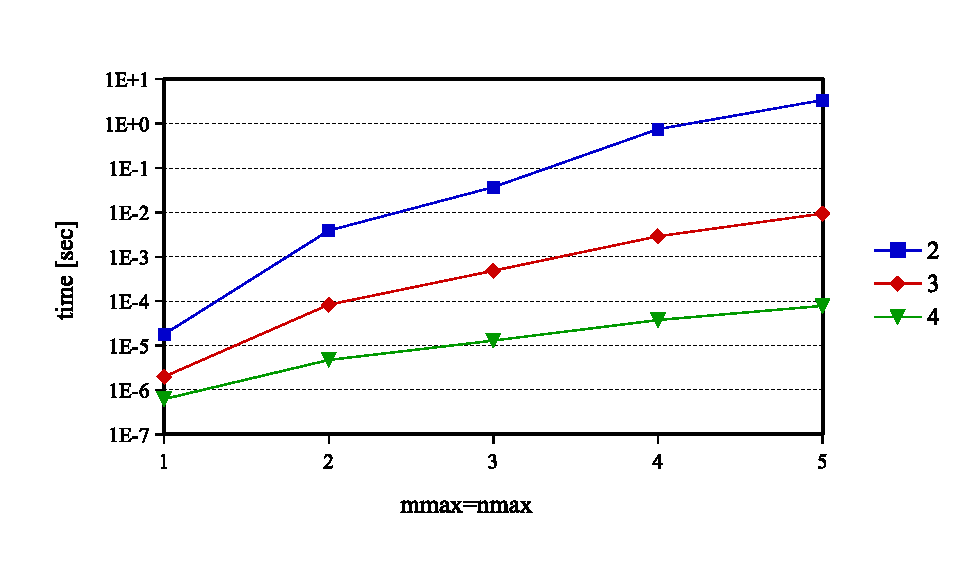
\includegraphics[bb=0bp 20bp 453bp 236bp,width=0.7\columnwidth]{_figure/results/k-kernel}
\par\end{centering}
\caption[Timing of a $k$-kernel]{Timing of a $k$-kernel (log scale)\label{fig:Timing-k-kernel}}
\end{figure}


\section{Entire iteration of $\mathcal{F}_{\mathrm{exc}}$ evaluation}

Apart from all the \texttt{\textbf{naive}} methods that will be discussed
in $\mathsection$\ref{subsec:Comparison-between-naive_standar},
figure \ref{fig:Entire-iteration} shows all the comparable \texttt{\textbf{convolution}}
timing data. We can see \texttt{\textbf{convolution\_standard}} is
the fastest algorithm, and \acs{OZ} equation is not the longest part
in the iteration. All the tests are performed for a $L=24$, $\mathrm{nfft}=72$
grid with 4 series: the three \texttt{\textbf{convolution}} methods
with $m_{\max}=n_{\max}$, and \texttt{\textbf{convolution\_standard}}
with $m_{\max}=5$, varying $n_{\max}$.

\begin{figure}[H]
\begin{centering}
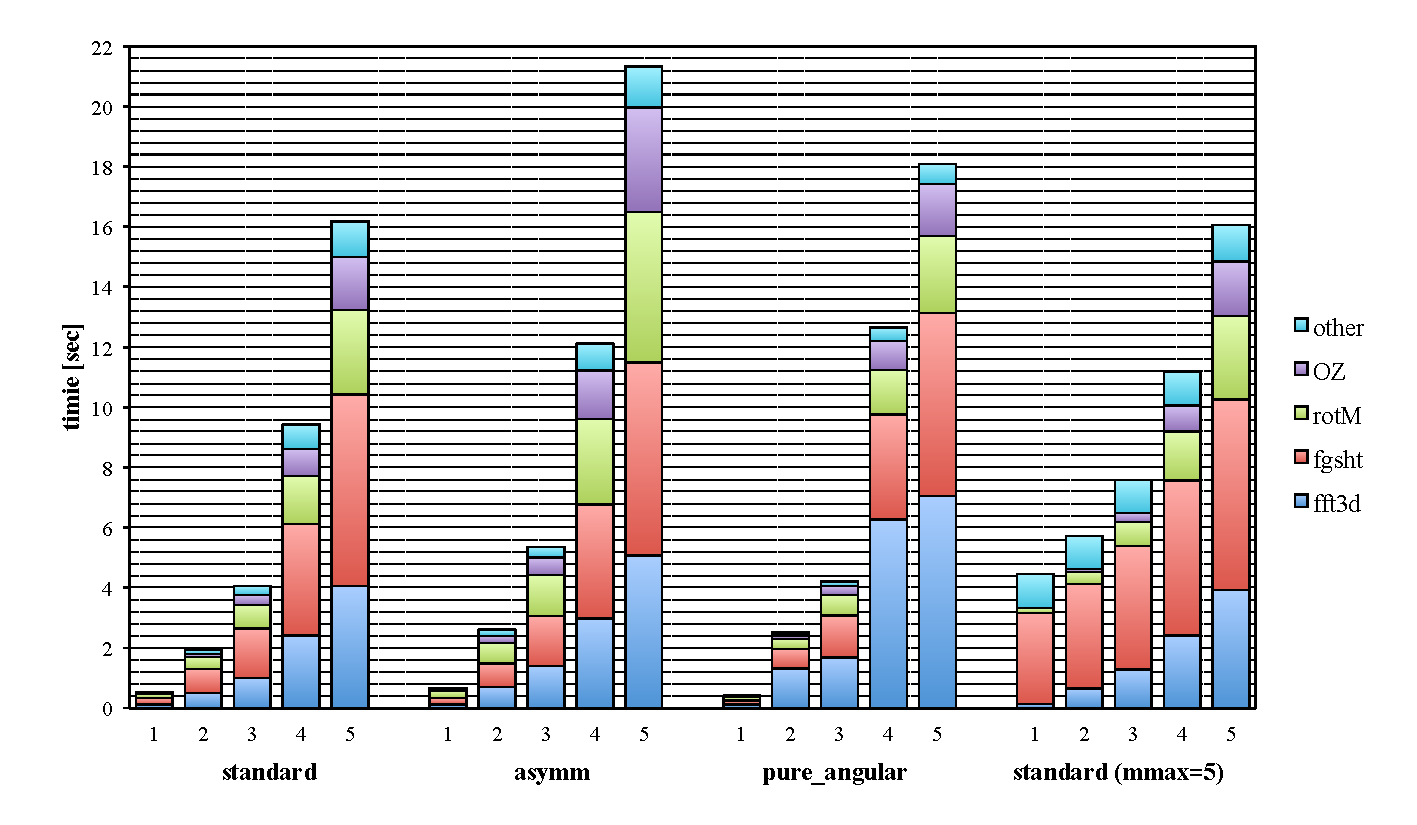
\includegraphics[width=0.9\columnwidth]{_figure/results/branch_perf}
\par\end{centering}
\caption[Entire iteration of $\mathcal{F}_{\mathrm{exc}}$ evaluation]{Entire iteration of $\mathcal{F}_{\mathrm{exc}}$ evaluation: timing
overall / decomposition of timing for 1 iteration evaluation\label{fig:Entire-iteration}}
\end{figure}


\subsection{``naive'' methods and ``convolution\_pure\_angular''\label{subsec:Comparison-between-naive_standar}}

The \texttt{\textbf{naive\_standard}}, \texttt{\textbf{naive\_interpolation}},
and \texttt{\textbf{convolution\_pure\_angular}} methods share the
same processes out of the $k$-kernel. Table \ref{tab:Timing-loop-k}
shows the timing of loop $k$ of these three methods. It indicates
that \texttt{\textbf{convolution\_pure\_angular}} takes far less time
than the other two methods, of which the loop $k$ takes time in the
same order of magnitude as the rest of iteration. And once $m_{\max}\geq2$,
\texttt{\textbf{naive\_interpolation}} is faster than \texttt{\textbf{naive\_standard}}.
Note that order 2 of \texttt{\textbf{naive\_interpolation}} can give
good results for a \acs{DCF} of $n_{\max}=5$. So in every case of
\texttt{\textbf{naive}} methods, \texttt{\textbf{naive\_interpolation}}
should be used. This verifies the conclusion of $k$-kernel test in
that the path (4) in figure \ref{fig:k-kernel} is the fastest.

\begin{table}[H]
\begin{centering}
\begin{tabular}{ccccc}
\toprule 
$m_{\max}$ & \texttt{\textbf{naive\_standard}} & \texttt{\textbf{naive\_interpolation}} & \texttt{\textbf{convo\_pure\_angular}} & \tableheadline{Other}\tabularnewline
\midrule
1 & 2.34 & 4.42 & 0.26 & 0.15\tabularnewline
2 & 365.95 & 209.12 & 1.09 & 1.43\tabularnewline
3 & 3295.00 & 752.70 & 2.37 & 1.85\tabularnewline
4 & too long & too long & 5.93 & 6.73\tabularnewline
5 & too long & too long & 10.36 & 7.73\tabularnewline
\bottomrule
\end{tabular}
\par\end{centering}
\caption[Timing of loop $k$]{Timing {[}sec{]} of loop $k$ of ``naive\_standard'', ``naive\_interpolation''
and ``convolution\_pure\_angular'', and the rest of iteration\label{tab:Timing-loop-k}}
\end{table}


\subsection{``convolution\_standard'' and ``convolution\_pure\_angular''}

The comparison of \texttt{\textbf{convolution\_standard}} and \texttt{\textbf{convolution\_pure\_angular}}
appears in figure \ref{fig:comparison-pure_angular}. Their difference
lies in the inversion of \acs{FFT} and \acs{FGSHT}. We can see the
other parts are almost identical, but the implementation of \acs{FFT}
is different in terms of time. Because in \texttt{\textbf{convolution\_standard}}
the number of \acs{FE} we need for \acs{FFT} is the number of projections,
and in \texttt{\textbf{convolution\_pure\_angular}} it is the number
of angular grid nodes. As there are fewer projections than angular
nodes, \texttt{\textbf{convolution\_standard}} reasonably takes less
time. The stair form of the \texttt{\textbf{pure\_angular}} curve
is due to the grid $\Psi$, which takes $\left\lfloor m_{\max}/2\right\rfloor $
points in the presence of $\mathrm{C}_{2v}$ symmetry. Projections
are less sensible.

\begin{figure}[H]
\begin{centering}
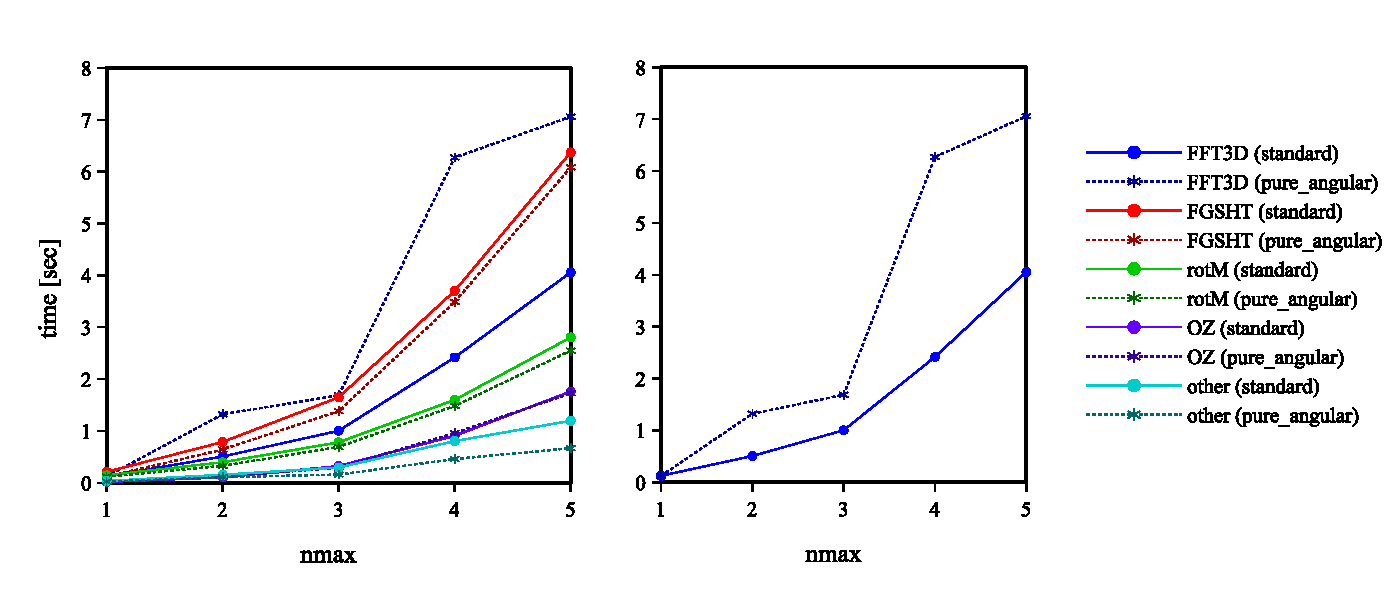
\includegraphics[bb=0bp 20bp 667bp 268bp,width=1\columnwidth]{_figure/results/pure_angular}
\par\end{centering}
\caption[Performance comparison of ``convolution\_standard'' and ``convolution\_pure\_angular'']{Performance comparison of \texttt{\textbf{convolution\_standard}}
and \texttt{\textbf{convolution\_pure\_angular\label{fig:comparison-pure_angular}}}}
\end{figure}


\subsection{``convolution\_standard'' and ``convolution\_asymm''}

We compare\texttt{\textbf{ convolution\_standard}} and \texttt{\textbf{convolution\_asymm}}
in figure \ref{fig:comparison-asymm}. The difference is that \texttt{\textbf{standard}}
calculates a half $k$ in the $k$-loop and \texttt{\textbf{asymm}}
calculates all $k$ in the $k$-loop. They share the same process
of \acs{FGSHT}; for the processes in a $k$-loop (rotM, OZ) \texttt{\textbf{asymm}}
always takes longer time. As in \texttt{\textbf{asymm}} we calculate
the \acs{FFT} for all the projections and in \texttt{\textbf{standard}}
we calculate only a half projections with $\mu\geq0$, the time consumed
by \acs{FFT} is also different.

\begin{figure}[H]
\begin{centering}
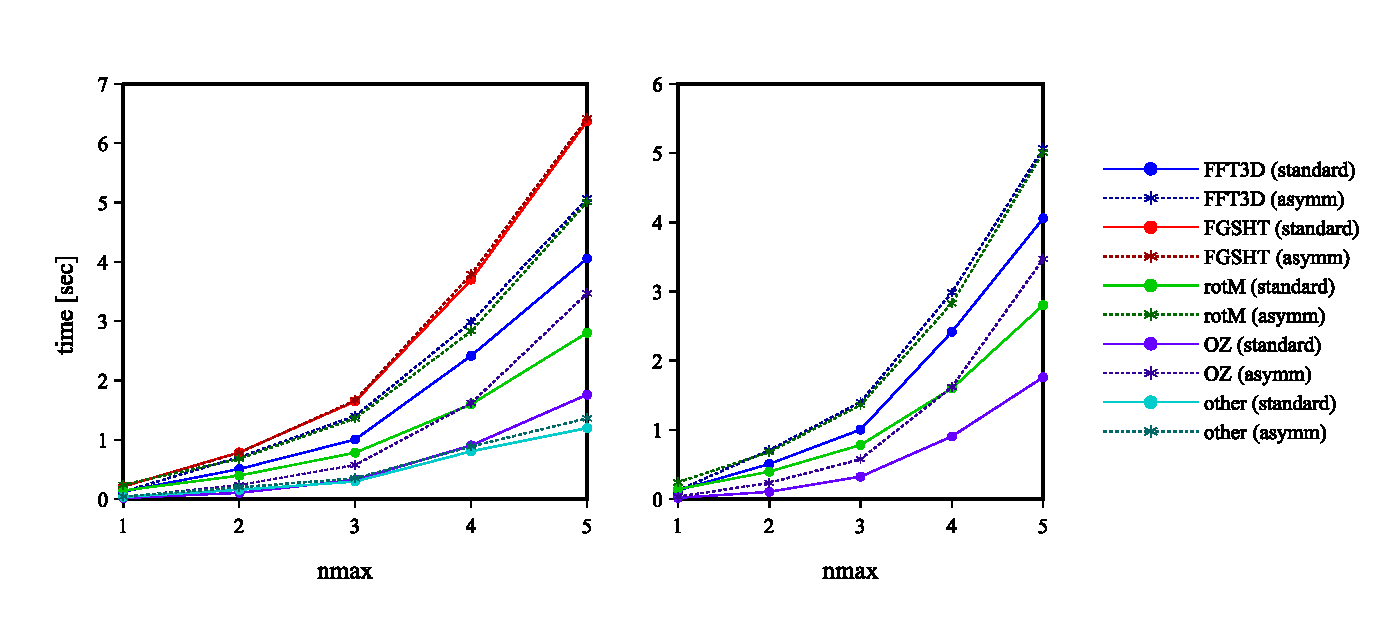
\includegraphics[bb=0bp 20bp 648bp 268bp,width=1\columnwidth]{_figure/results/asymm}
\par\end{centering}
\caption[Performance comparison of ``convolution\_standard'' and ``convolution\_asymm'']{Performance comparison of \texttt{\textbf{convolution\_standard}}
and \texttt{\textbf{convolution\_asymm\label{fig:comparison-asymm}}}}
\end{figure}


\subsection{Distinction of $m_{\max}$ and $n_{\max}$}

The comparison of $m_{\max}=n_{\max}$ and $m_{\max}=5$ for\texttt{\textbf{
convolution\_standard}} is shown in figure \ref{fig:comparison-nmax}.
We see that the choice of quadrature order $m_{\max}$ only affects
the \acs{FGSHT} process and the lecture/storage of density variable
(other). The time taken by extra order $m_{\max}$ is not cost-free,
as discussed in last section, it is fully recommended to use $m_{\max}=n_{\max}$.

\begin{figure}[H]
\begin{centering}
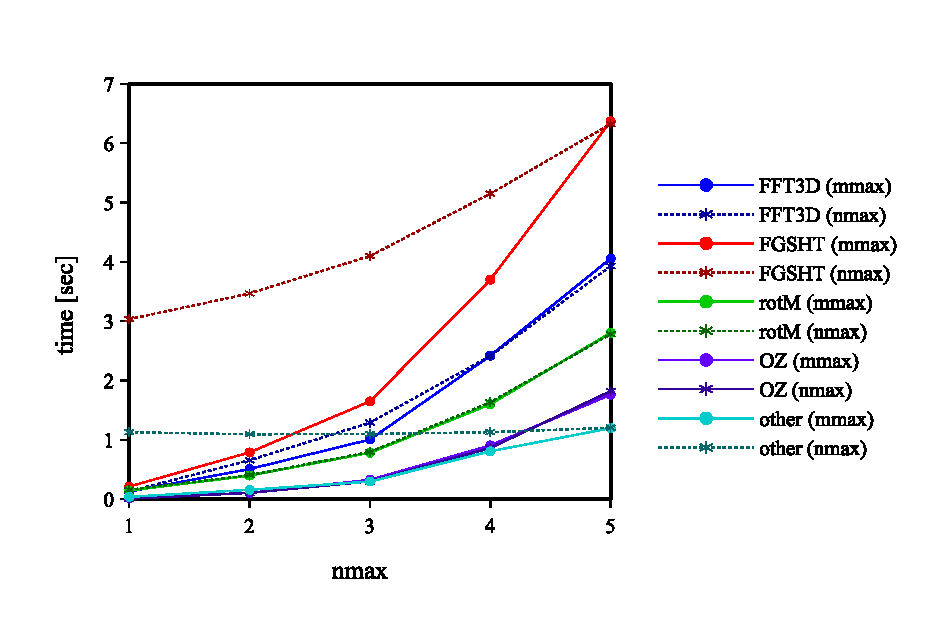
\includegraphics[bb=0bp 20bp 639bp 268bp,width=1\columnwidth]{_figure/results/nmax}
\par\end{centering}
\caption[Performance comparison of ``convolution\_standard'' for $m_{\max}=n_{\max}$
and $m_{\max}=5$]{Performance comparison of \texttt{\textbf{convolution\_standard}}
for $m_{\max}=n_{\max}$ and $m_{\max}=5$\label{fig:comparison-nmax}}
\end{figure}


\section{Global view of the code performance}

\begin{figure}[H]
\begin{centering}
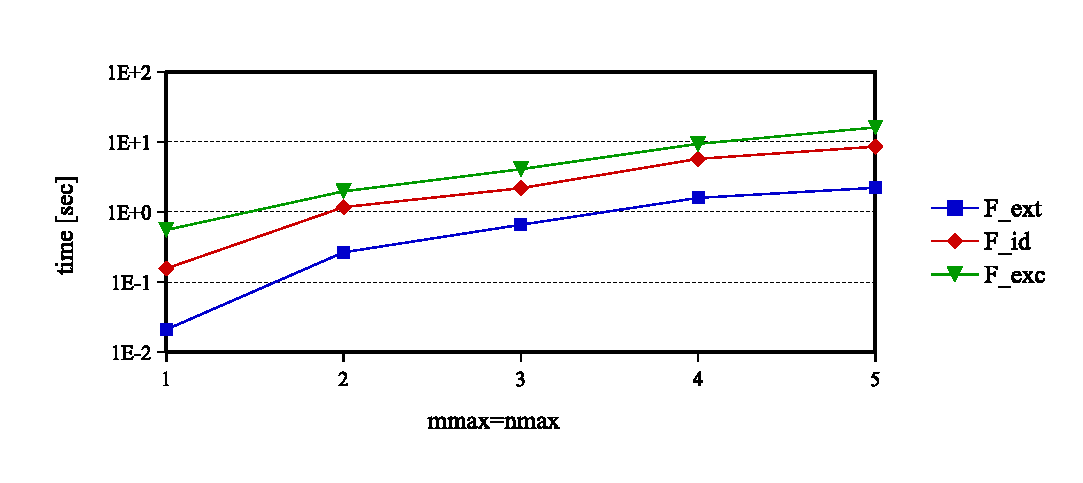
\includegraphics[bb=0bp 20bp 453bp 236bp,scale=0.7]{_figure/results/global_perf}
\par\end{centering}
\caption[Timing of the whole $\mathcal{F}$ iteration]{Timing of the whole $\mathcal{F}$ iteration with $\mathrm{nfft}/L=72/24$
grid (log scale)}
\end{figure}

Note that this is for an ion solute. $\mathcal{F}_{\mathrm{ext}}$
can be very slow if the solute have a very complex form.

We can see that \texttt{\textbf{convolution\_standard}} is the fastest.
The \texttt{\textbf{convolution}} methods are orders of magnitude
faster than \texttt{\textbf{naive}} methods. The evaluation of $\mathcal{F}_{\mathrm{exc}}$
is at the same order of magnitude than other two terms and the same
dependency on angular grid.
